\documentclass{beamer}

% Prep browser tabs:
% - cgran.org
% - PyBOMBS github (start at manual)
% - A PyBOMBS recipe from gr-recipes
% - Guided tutorials

\usetheme{GNURadio}
\usepackage{palatino}
\usepackage{xcolor}
\usepackage{tikz}
\usepackage[utf8]{inputenc}
\usepackage{listings}
\usepackage{alltt}

\title{PyBOMBS \& CGRAN --- An Update}
\institute{Martin Braun}

\date{GNU Radio Conference 2016}

\graphicspath{{./}}
\DeclareGraphicsExtensions{.png,.pdf}

% Comment this out to not have a TOC every time you have a \section:
\AtBeginSection[] {%
  \begin{frame}
    \frametitle{Outline}
    \tableofcontents[currentsection]
  \end{frame}
}

\begin{document}

% Title page:
\frame{\titlepage}

\begin{frame}
  \frametitle{CGRAN\@: A Reminder, and a preview}
  \begin{itemize}
    \item Where can you find all the incredible GNU Radio projects?
    \item \texttt{www.cgran.org}
    \item As a project maintainer, your project could be listed here!
    \item Coming soon: \texttt{pybombs}-protocol will auto-install modules
  \end{itemize}
\end{frame}


\section{Installing GNU Radio and OOTs}
\begin{frame}
  \frametitle{Top 4 easiest ways to install GNU Radio}
  \begin{enumerate}
    \item The GNU Radio Live DVD
    \item<2-> \texttt{apt install gnuradio} --- use your package manager, whatever that is
    \item<3-> PyBOMBS (Version 2!)
    \item<4-> Source Builds
  \end{enumerate}
    \hspace{3em}
    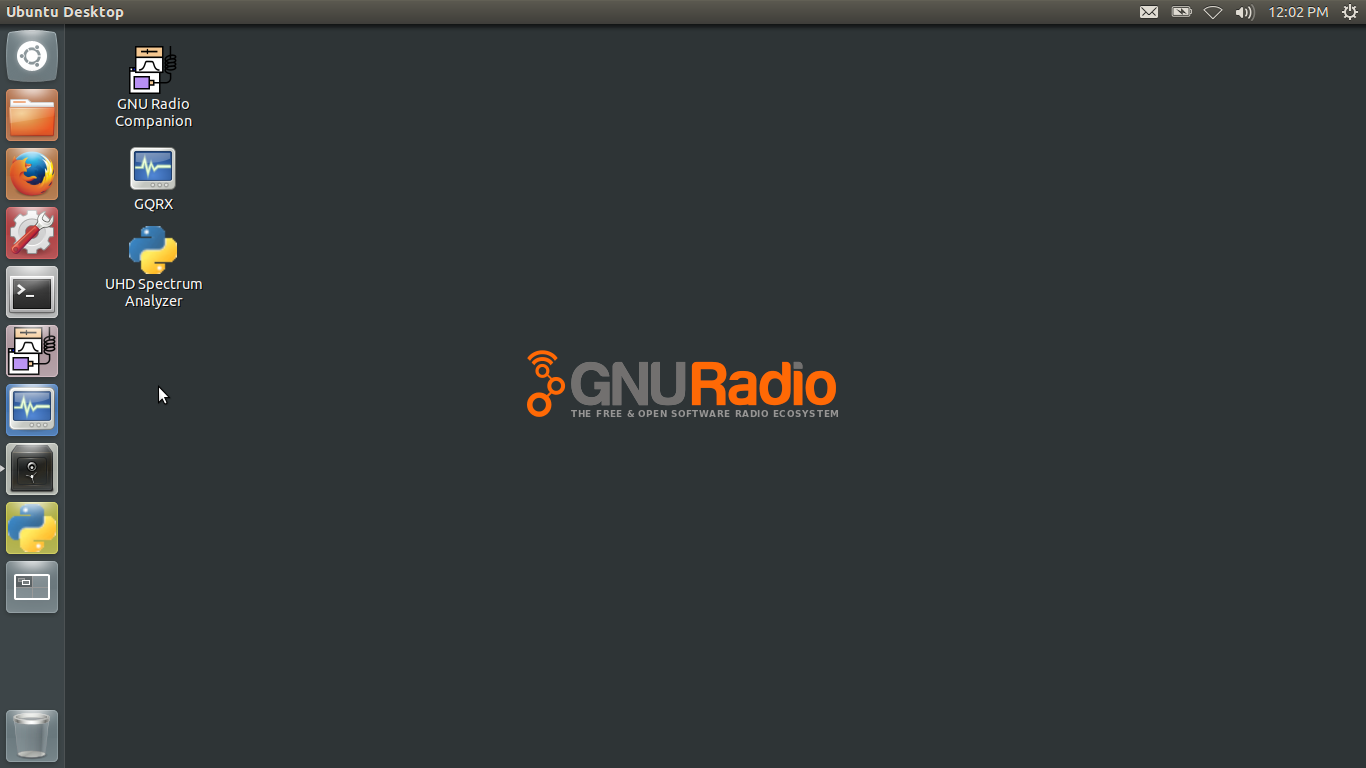
\includegraphics[height=5em]{grlivedvd}
    \hspace{1em}
    \includegraphics<3->[height=5em]{pybombs_logo}
    \hspace{1em}
    \includegraphics<4->[height=5em]{srcbuild}
\end{frame}

\begin{frame}
  \frametitle{PyBOMBS\@: What you will need}
  \begin{itemize}
    \item A Linux or Mac box (one day we'll have Windows covered, but not today)
    \item Fedora, Ubuntu, CentOS, Debian, and probably many other distros fine
    \item Python 2.7
    \item<2-> And what else\ldots
    \item<3-> Nope, that's it! (Maybe some hardware?)
  \end{itemize}
\end{frame}

\begin{frame}
  \frametitle{Getting started with PyBOMBS}
  \begin{itemize}
    \item Install PyBOMBS\@: \texttt{pip install pybombs}
    \item Optionally install PyBOMBS GUI\@: \texttt{pip install pybombs-qtgui}
    \item Install recipes:
      {\footnotesize{%
\begin{alltt}
\$ pybombs recipes add gr-recipes  \\
git+https://github.com/gnuradio/gr-recipes.git \\
\$ pybombs recipes add gr-etcetera\\
git+https://github.com/gnuradio/gr-etcetera.git
\end{alltt}
}}
    \item Now let's install GNU Radio and all dependencies:
    \item {\footnotesize{\texttt{pybombs prefix init -a default -R gnuradio-default /home/mbr0wn/prefix/gnuradio}}}
  \end{itemize}
\end{frame}

\section{PyBOMBS concepts}
\begin{frame}
  \frametitle{Why do I need a \emph{prefix}?}
  \begin{itemize}
    \item Standard Unix way (since probably even Marcus Leech started) is to install software either into \texttt{/usr} or \texttt{/usr/local}.
    \item Self-compiled software would default into the latter
    \item This is simple and understood, but has some problems:
    \begin{itemize}
      \item No standard way to uninstall hand-installed software
      \item Only one installation at a time possible
      \item Requires admin (sudo) privileges
    \end{itemize}
    \item So how about we install it into some random directory in our home?
    \item \texttt{/home/mbr0wn/prefix/gnuradio} --- The prefix!
    \item Solves all the problems above, except we now need to tell the system where to look for stuff (\emph{environment variables} need setting)
  \end{itemize}
\end{frame}

\begin{frame}
  \frametitle{What makes a PyBOMBS prefix special?}
  \begin{itemize}
    \item May have a \texttt{.pybombs} subdirectory, which stores local special configurations.
    \item All config files are YAML format.
    \item Use \texttt{pybombs prefix init} to create the prefix directory.
  \end{itemize}
\end{frame}


\begin{frame}
  \frametitle{\texttt{pybombs prefix init}}
  \begin{itemize}
    \item Show me that command again:
      \begin{alltt}
      pybombs\\
          prefix init \\
          --alias default \\
          --recipe gnuradio-default \\
          /home/mbr0wn/prefix/gnuradio
      \end{alltt}
    \item Aah, I get it now. We install into \texttt{prefix/gnuradio}, and we use the rules defined in \texttt{gnuradio-default}.
    \item We call such definitions a \emph{recipe}.
  \end{itemize}
\end{frame}

\begin{frame}
  \frametitle{So\ldots recipes?}
  \begin{itemize}
    \item Remember the \texttt{pybombs recipe add} commands?
    \item These are part of most people's installation. (See PyBOMBS manual).
    \item Will install all default recipes.
    \item Let's take a quick look at one of those.
    \item Like all PyBOMBS config files, in YAML format.
  \end{itemize}
\end{frame}

\begin{frame}
  \frametitle{How do I install things then?}
  \begin{itemize}
    \item \texttt{pybombs install [-p PREFIX ] PACKAGE}
    \item Let me show you.
    \item \texttt{PREFIX} is either an alias, or a full path.
  \end{itemize}
\end{frame}

\begin{frame}
  \frametitle{And how do I run GNU Radio now?}
  \begin{itemize}
    \item First, initialize your prefix of choice:
    \item \texttt{source \$PREFIX/setup\_env.sh}
    \item You're good. Run: \texttt{gnuradio-companion} if you don't believe me.
    \item You can initialize any number of prefixes at once (only one per shell, though).
    \item Clicky launchers also work fine.
  \end{itemize}
\end{frame}

\begin{frame}
  \frametitle{Why is PyBOMBS accessing my system?}
  \begin{itemize}
    \item PyBOMBS is not a container replacement.
    \item It will use any means to get your system ready to build software (e.g., GNU Radio).
    \item Your system's package manager is one of those means.
    \item It might need elevated privileges. This is normal.
    \item Here's a nice trick: \texttt{pybombs install --deps-only gnuradio}
  \end{itemize}
\end{frame}

\section{Out-of-tree Modules}
\begin{frame}
  \frametitle{Out-of-tree Modules}
  \begin{itemize}
    \item GNU Radio comes with a lot of blocks, but a lot of the value comes from the ability to extend it.
    \item Other people like to share their extensions to GNU Radio!
    \item If they're particularly awesome, they're on \texttt{www.cgran.org}!
    \item Side note: Making OOTs is really easy. Just use \texttt{gr\_modtool}!
    \item See Guided Tutorials on the GNU Radio wiki.
  \end{itemize}
\end{frame}

\begin{frame}
  \frametitle{PSA for content producers}
  \begin{itemize}
    \item If you're a producer of GNU Radio-related products or projects, listen up!
    \item Please consider using PyBOMBS\@.
    \item We're trying to consolidate installation methods.
    \item Create your own recipe repository if you have anything else than a single standard recipe.
    \item Include manifests in your OOTs so we can source them for CGRAN\@.
  \end{itemize}
\end{frame}

\begin{frame}
  \frametitle{SDKs/Cross-compiling with PyBOMBS}
  \begin{itemize}
    \item PyBOMBS for embedded devices is (fairly) well supported
    \item \ldots{}if the recipes exist
    \item Just FYI\@: PyBOMBS method conflicts with what some embedded people think is the right way to go
  \end{itemize}
\end{frame}

\section{Conclusion}
\begin{frame}
  \frametitle{FAQ}
  \begin{itemize}
    \item Q\@: Why not just use the package manager?\\A\@: You can use both. PyBOMBS will give you the most up-to-date code, and works for most OOTs.
    \item Q\@: Can't I just do this all by hand?\\A\@: Knock yourself out!
    \item Q\@: Will PyBOMBS help me cross-compile? A\@: It'll basically do all the work for you---if you have proper recipes.
    \item Q\@: Will you make PyBOMBS work on my system/OS\@? A\@: Yes, by gladly accepting your patches!
    \item Q\@: Bugfixes/contributions? A\@: github!
    \item Q\@: Why didn't you use an existing tool instead of writing PyBOMBS\@? A\@: Many good reasons.
  \end{itemize}
\end{frame}

\begin{frame}
  \frametitle{Conclusion}
  \begin{itemize}
    \item PyBOMBS is awesome and can save you time.
    \item Sysadmin-friendly (I believe).
    \item All our cool stuff is on CGRAN\@. You want to be on CGRAN, too.
    \item Thanks to all contributors, users and bugfixers!
  \end{itemize}
\end{frame}

\end{document}
